\documentclass[a4paper,14pt]{extarticle}
\usepackage[T2A]{fontenc} % кодировка
\usepackage[utf8]{inputenc} % кодировка исходного текста
\usepackage[english,russian]{babel}
\usepackage{mathtools}
% \usepackage{psfrag,pstricks}
\usepackage{makeidx}
\usepackage{graphicx}
\usepackage{indentfirst}
\usepackage{siunitx}

\title{Анализ популяционной модели Базыкина <<хищник-жертва>>}
\author{ Белов Тимофей Викторович \and Крутовский Данил Александрович }
\date{\today}

\makeindex
\begin{document}
\maketitle

\newpage
\tableofcontents

\newpage
\section{Введение}
Построение и анализ математических моделей являются важными инструментами научного исследования различных явлений, в том числе физических и  химических. В настоящее время существует возможность эффективно применять применять методы исследования моделей, опирающиеся на применение компьютерных технологий для постановки численных экспериментов и обработки их результатов. 
В частности представляет интерес исследование с помощью таких методов моделей билогических процессов, каковой является и популяционная модель Базыкина <<хищник-жертва>>. 

Модель хищник-жертва – это особая взаимосвязь хищника с жертвой, в результате которой выигрывают оба. Выживают наиболее здоровые и приспособленные особи к условиям среды обитания, т.е. все это происходит благодаря естественному отбору.
В той среде где нет возможности для размножения, хищник рано или поздно уничтожит популяцию жертвы, в последствии чего вымрет и сам.

Данная модель является обощением модели Лотки-Вольтерра, учитывающей важные биологические факторы: насыщение хищников, внутривидовую конкуренцию. Модель имеет большое значение для понимания процессов, происходящих в различных популяционных системах, их биологических потенциалов и влиянии друг на друга.


\section{Постановка задачи работы}
Целью работы является исследование детерминированных и стохастических свойств математической модели <<хищник-жертва>> Базыкина. В работе предполагается проведение бифуркационного анализа детерминированной системы и построение бифуркационной диаграммы, анализ восприимчивости к случайным возмущениям на основе прямого численного моделирования.

\section{Описание модели}
 Модель Базыкина <<хищник-жертва>> воспроизводит периодический колебательный режим, возникающий в результате межвидовых взаимодействий в природе:


$$\begin{cases}
  ̇\dot x = x-cx^2-a\dfrac{xy}{1+x}\\
  \dot y = -y + b\dfrac{xy}{1+x},
\end{cases} (1) $$

где:

$x$ ~--~ численность жертв

$y$ ~--~ численность хищников

$a$ ~--~ коэфицент сметности жертвы при столкновении с хищником

$b$ ~--~ коэфицент насыщаемости хищника при столкновении с жертвой

$c$ ~--~ коэфицент внутривидовой конкуренции между жертвами

$a, b, c > 0$

$a=2, c=0.1, b > 1$


\newpage
\section{Детерминированные свойства модели}
Для исследования детерминированных свойств модели воспользуемся теоремой Гробмана-Хартмана, утверждающей, что в окрестности неподвижной точки поведение исследуемой системы совпадает с поведением ее линеаризации. Из этого следует, что в некоторой окрестности неподвижной точки фазовый портрет системы (1) совпадает с портретом линеаризованной системы, в случае, если система (1) имела портрет типа <<узел>>, <<фокус>> или <<седло>>.

\subsection{Точки покоя и их устойчивоть}

Вычислим точку покоя для исследуемой модели из условий равенства нулю производных:
$$\begin{cases}
  0 = x-cx^2-a\dfrac{xy}{1+x}\\
  0 = -y + b\dfrac{xy}{1+x}
\end{cases}$$
Решив систему, получим следующие точки покоя:
$$ M_0 = \left(0,0 \right) $$
$$ M_1 = \left(\dfrac{1}{c}, 0 \right) $$ 
$$ M_2 = \left(\dfrac{1}{b-1}, \dfrac{(b-c-1)b}{a(b-1)^2} \right) $$
Составим матрицу Якоби: 
$$\left(
\begin{matrix}
-2cx+1-\dfrac{ay}{(x+1)^2} & -\dfrac{ax}{x+1}\\
\dfrac{by}{(x+1)^2} & -1 + \dfrac{bx}{x+1}
\end{matrix}
\right)$$
Характеристический многочлен матрицы: 
$$ \lambda^2 + (2cx+\frac{ay-bx(x+1)}{(x+1)^2})\lambda + (2cx+\frac{ay+bx(x+1)}{(x+1)^2}) - (2cx\frac{bx}{x+1} + 1)$$

Рассмотрим точки покоя по отдельности:

В точке $M_0$ корни характеристического многочлена имеют вид $\lambda = \pm 1$. Из этого делаем вывод, что тип фазового портрета - $Saddle$.

В точке $M_1$:$b \in$
$\left[ 
\begin{array}{l}
  (1, 1 + c) \Rightarrow Stable\ Node\\
  (c + 1, +\infty) \Rightarrow Saddle \\
\end{array} 
\right.$

В точке $M_2$:$b \in$
$\left[ 
\begin{array}{l}
 \left(1, c+1 \right) \Rightarrow Saddle \\
 \left(c+1, \frac{c}{2(\sqrt2-1)}+1\right) \Rightarrow Node\ (stable) \\
 \left(\frac{c}{2(\sqrt2-1)}+1, \frac{2}{1 - c}-1\right) \Rightarrow  Focus\ (stable) \\
 \left(\frac{2}{1 - c}-1, +\infty \right) \Rightarrow Focus\ (unstable)
\end{array} 
\right.$


\subsection{Бифуркационные диаграммы}
\subsubsection{Типы фазовых портретов}

В точке $M_0$ вне зависимости от параметров системы тип фазового портрета всегда будет «Седлом».

В точке $M_1$:$b \in $
$\left[ 
\begin{array}{l}
  (1, 1 + c) \Rightarrow Stable\ Node\\
  (c + 1, +\infty) \Rightarrow Saddle \\
\end{array} 
\right.$
\begin{figure}[!h]
\centering
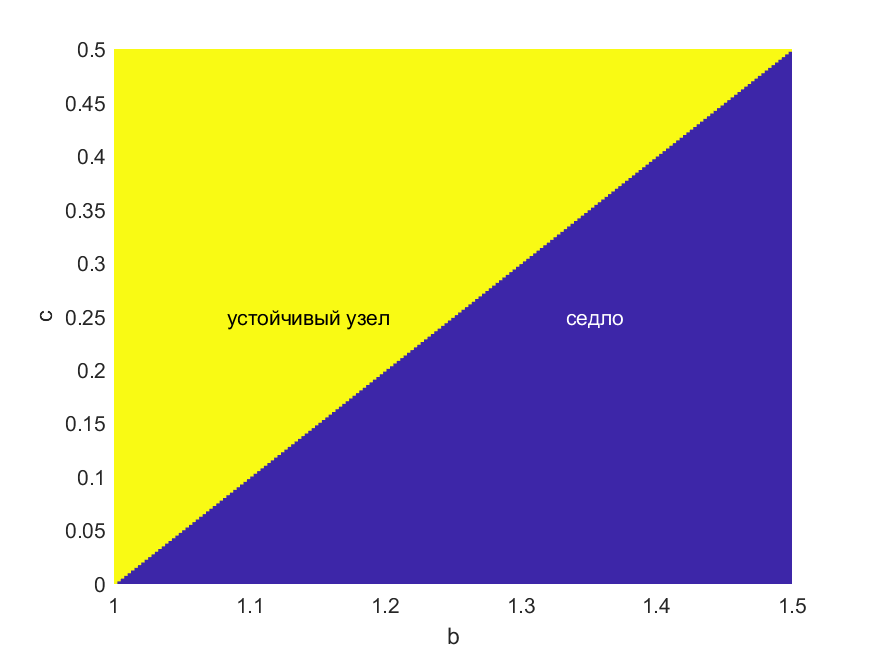
\includegraphics[scale=0.7]{Labs/m1_portret_types.png}
\caption{Двупараметрическая бифуркационная диаграмма для $M_1$}
\label{bif_m1}
\end{figure}


В точке $M_2$:$b \in$
$\left[ 
\begin{array}{l}
 \left(1, c+1 \right) \Rightarrow Saddle \\
 \left(c+1, \frac{c}{2(\sqrt2-1)}+1\right) \Rightarrow Node\ (stable) \\
 \left(\frac{c}{2(\sqrt2-1)}+1, \frac{2}{1 - c}-1\right) \Rightarrow  Focus\ (stable) \\
 \left(\frac{2}{1 - c}-1, +\infty \right) \Rightarrow Focus\ (unstable)
\end{array} 
\right.$
\begin{figure}[!h]
\centering
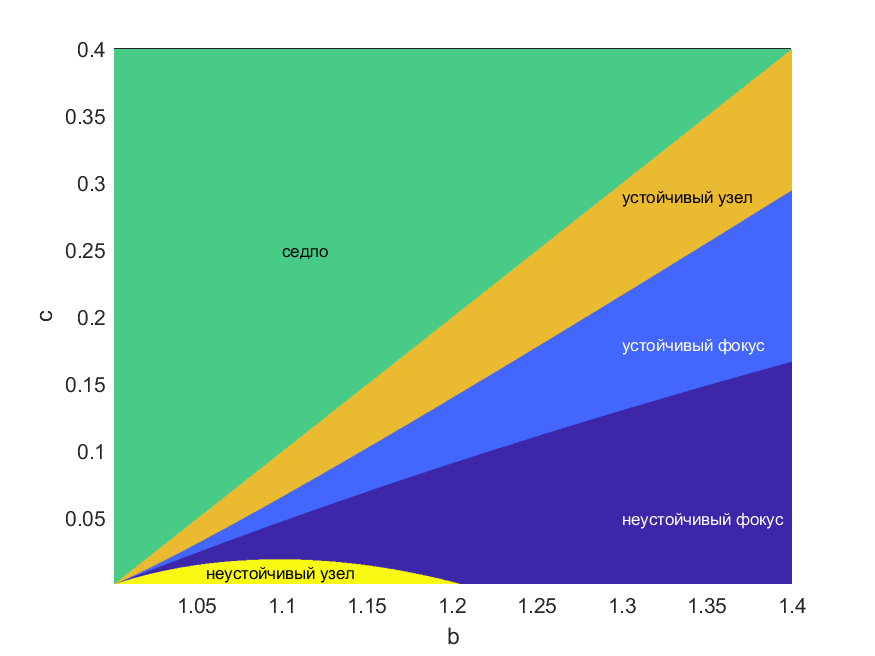
\includegraphics[scale=1]{Labs/m2_portret_types.png}
\caption{Двупараметрическая бифуркационная диаграмма для $M_2$}
\label{bif_m2}
\end{figure}

\newpage
\subsubsection{Аттракторы и репеллеры}
Построим бифуркационную диаграмму с описанием аттракторов(репеллеров), зафиксировав параметры $a=2, c=0.1$:


\begin{figure}[!h]
\centering
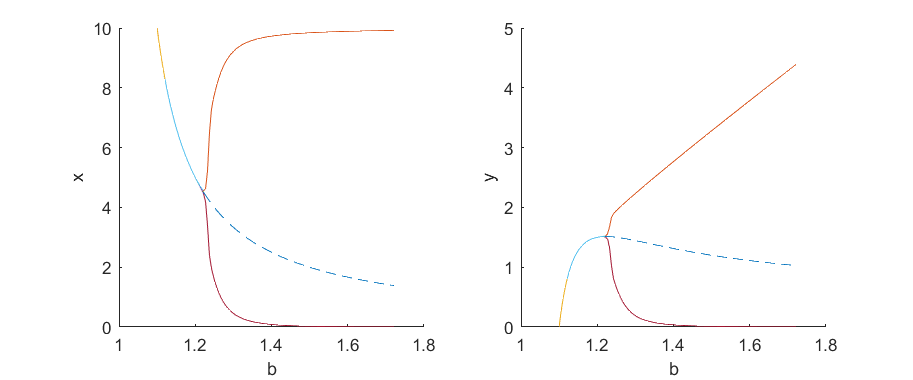
\includegraphics[width=\linewidth]{Labs/sups.png}
\caption{Супремумы координат
X и Y}
\label{attr_repell}
\end{figure}

Анализ интервалов по параметру $b$:
\begin{itemize}
\item На $[1.1 = 1 + c, \frac{2}{1 - c}-1 = \frac{11}{9}]$ равновесие устойчиво и является единственным аттрактором.
\item На $[\frac{11}{9}, 1.7]$ предельный цикл является единственным аттрактором.
\end{itemize}

В нашей системе, $M_0$ и $M_1$ являются <<седлами>>, они и задают минимум и максимум по координате $x$ и зафиксированы при больших параметрах $b$. Также, при росте $b$ наблюдается рост предельного цикла по координате $y$. Таким образом, мы можем быть уверены, что на бесконечности для обеих координат при данном $c$ сохранится поведение, как на интервале $[\frac{11}{9}, 1.7]$

Весь интервал является зоной моностабильности.

\newpage
\subsubsection{Атлас фазовых портретов}

Зеленая зона:
Точка $M_2$ в данной конфгурации не существует

$M_1$~--~ устойчивый узел.
\begin{figure}[!h]
\centering
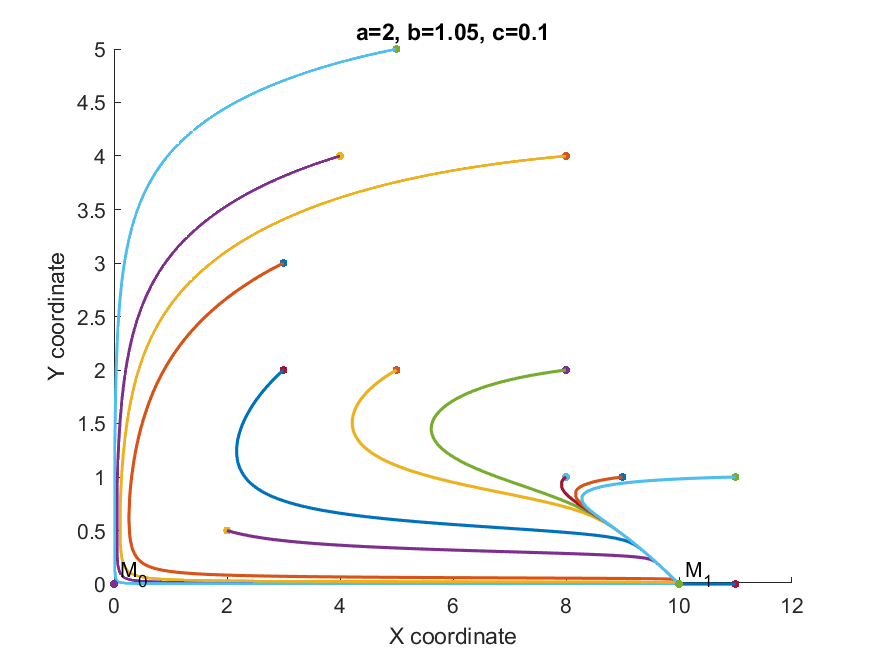
\includegraphics[width=\linewidth]{Labs/portret_1.png}
\caption{$a = 2;b \in (1, 1 + c);c = 0.1$}
\label{prt1}
\end{figure}

\newpage
Переход между зеленой и оранжевой областями:
$M_1$=$M_2$~--~ устойчивые узлы.
\begin{figure}[!h]
\centering
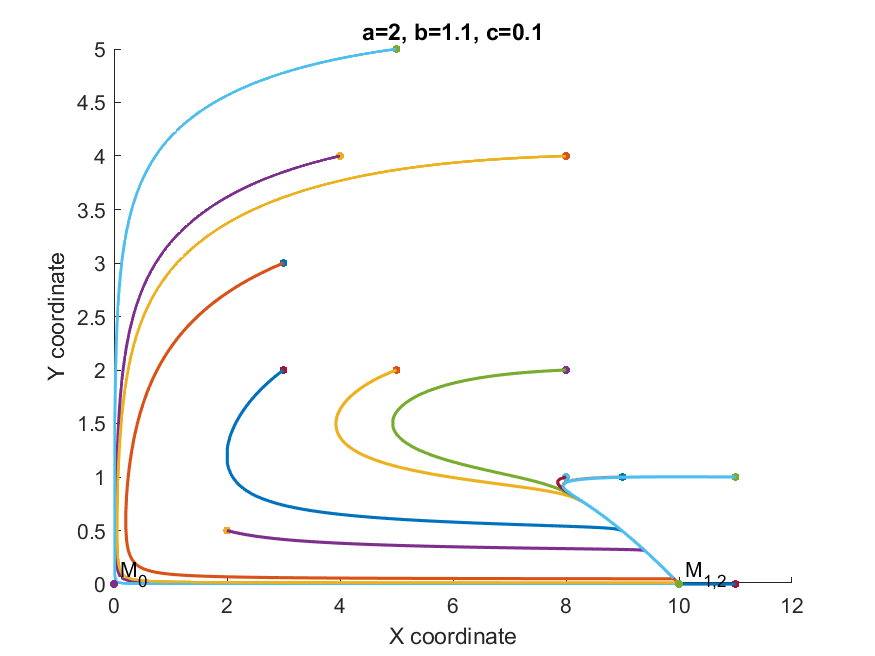
\includegraphics[width=\linewidth]{Labs/portret_2.png}
\caption{$a = 2;b = 1 + c;c = 0.1$}
\label{prt2}
\end{figure}

\newpage
Оранжевая зона:
$M_2$~--~ устойчивый узел.
\begin{figure}[!h]
\centering
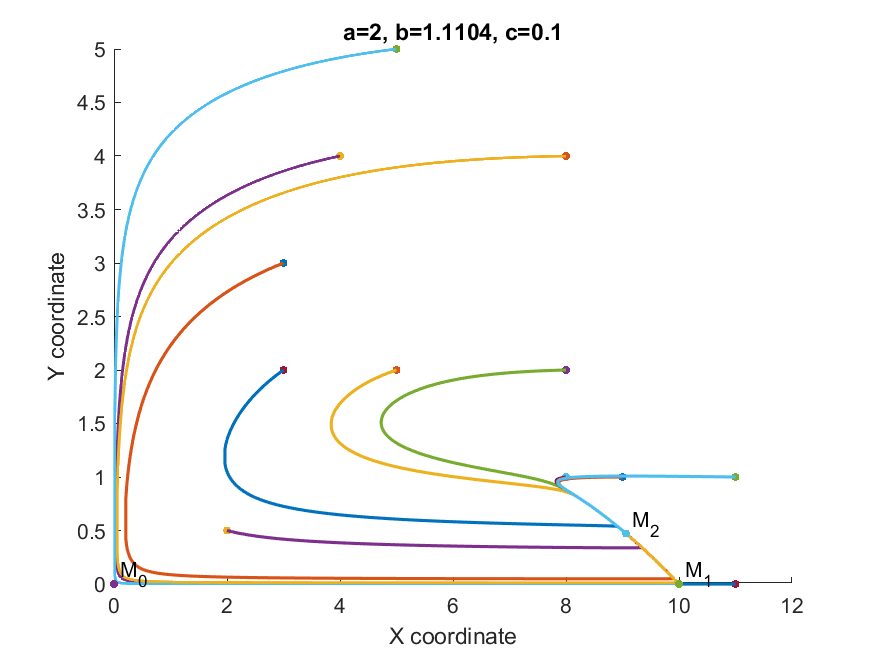
\includegraphics[width=\linewidth]{Labs/portret_3.png}
\caption{$a = 2;b \in (1 + c, \frac{c}{2(\sqrt2-1)}+1];c = 0.1$}
\label{prt3.1}
\end{figure}

\newpage
Переход между зонами захватывается оранжевой зоной, поэтому его пропускаем.
Голубая зона:
$M_2$ ~--~ устойчивый фокус.
\begin{figure}[!h]
\centering
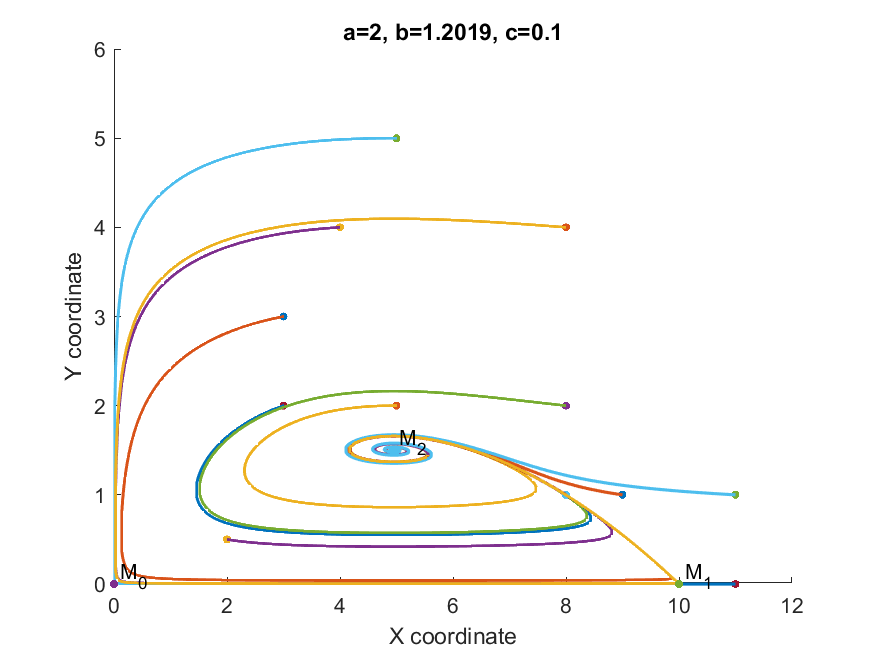
\includegraphics[width=\linewidth]{Labs/portret_4.png}
\caption{$a = 2; b \in (\frac{c}{2(\sqrt2-1)}+1, \frac{2}{1 - c}-1); c = 0.1$}
\label{prt4}
\end{figure}

\newpage
Переход между голубой и синей областями:
$M_2$ ~--~ центр.
\begin{figure}[!h]
\centering
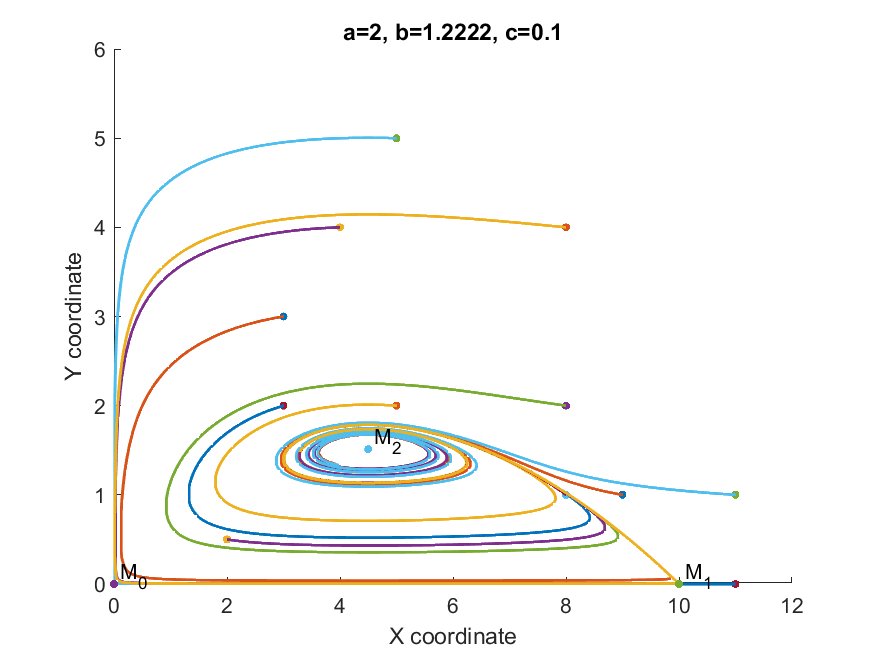
\includegraphics[width=\linewidth]{Labs/portret_5.png}
\caption{$a = 2; b = \frac{2}{1 - c}-1; c = 0.1$}
\label{prt5}
\end{figure}

\newpage
Синяя зона:
В данной зоне впервые наблюдается появление предельного цикла.

$M_2$ ~--~ неустойчивый фокус.
\begin{figure}[!h]
\centering
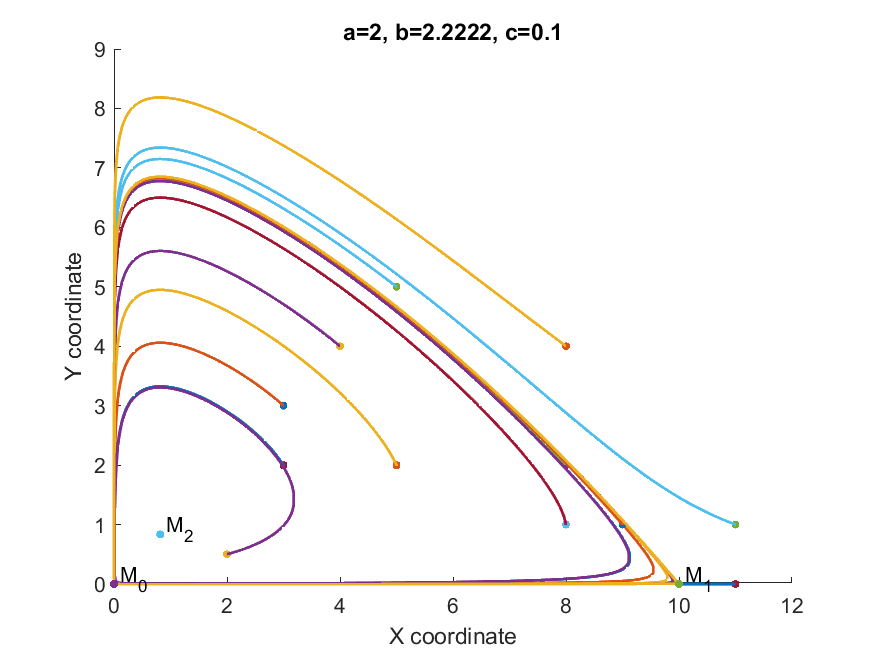
\includegraphics[width=\linewidth]{Labs/portret_6.png}
\caption{$a = 2; b \in (\frac{2}{1 - c}-1, +\infty); c = 0.1$}
\label{prt6}
\end{figure}

\newpage
Жёлтая зона:
Стоит заметить, что для значений параметров $b$ и $c$, удовлетворяющим жёлтой зоне, предельный цикл сильно увеличивает свои размеры (100 к 10 для координаты $x$ и 20 к 5-8 для $y$).

$M_2$ ~--~ неустойчивый узел.
\begin{figure}[!h]
\centering
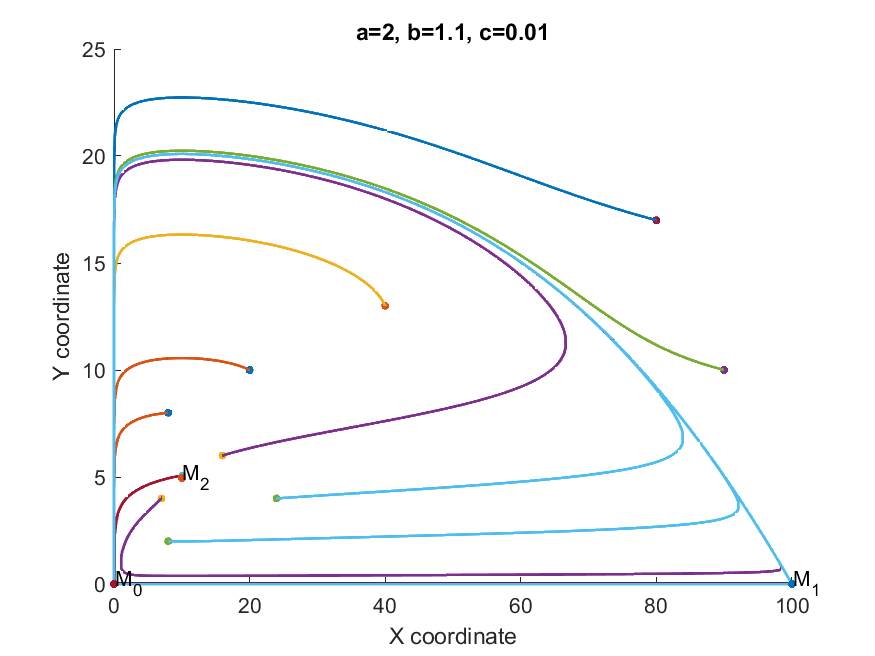
\includegraphics[width=\linewidth]{Labs/portret_7.png}
\caption{$a = 2; b = 1.1; c = 0.01$}
\label{prt7}
\end{figure}

\newpage
\subsection{Предельные циклы}

Точка $\widetilde{x}$ фазовой плоскости называется предельной точкой траектории $X = \varphi \left(t\right)$, если существует последовательность $t_n \to +\infty$, либо $t_n \to -\infty$ такая, что $\varphi \left(t_n\right) \to \widetilde{x}$. Предельным множеством траектории называется множество всех её предельных точек. Предельный цикл - это замкнутое (периодическое) решение системы, представляющее собой предельное множество некоторой её траектории. Для случая фазовой плоскости известно (по т. Пуанкаре~--~Бендиксона), что предельное множество любой траектории представляет собой либо точку покоя, либо предельный цикл, либо предельный полицикл. В случае, когда точка покоя системы неустойчива, на фазовой плоскости присутствуют предельные циклы.

Для нахождения предельных циклов использовался метод Рунге~--~Кутта с размером шага $h = \num{1e-3}$


\newpage
\subsubsection{Орбиты}
Следующие изображения демонстрируют нам изменение предельный цикл в зависимости от параметров $b$ и  $c$. Можно заметить, что при росте параметра $b$ предельный цикл принимает более треугольную форму, а при росте $c$ - округляется. 
На изображениях синей точкой представлена точка покоя(фокус), оранжевой - точка старта.
\begin{figure}[!h]
\centering
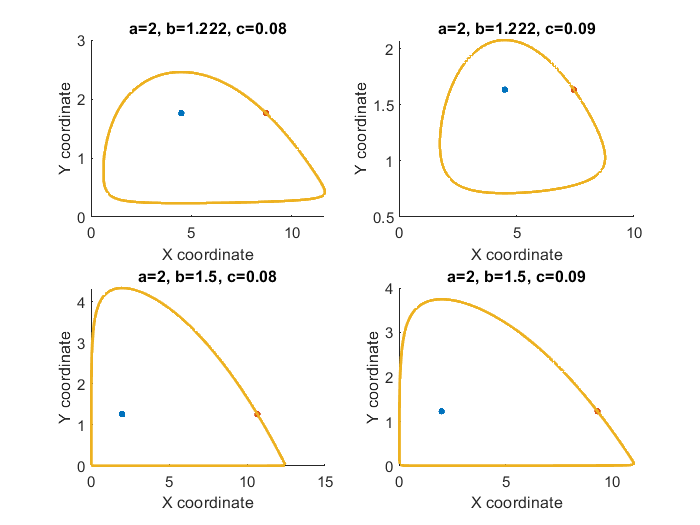
\includegraphics[scale=0.8]{Labs/four_cycles.png}
\caption{Несколько циклов}
\label{cycles}
\end{figure}

\newpage
\subsubsection{График периода}
Посмотрим на график периода цикла в зависимости от параметра $b$. Можно заметить, что при $b \approx 1.4$ и $b \approx 1.6$ наблюдаются перегибы кривой. 

Предположение: Во время первого перегиба один <<катет>> цикла окончательно прижимается к оси $OX$ и фиксирует свои размеры, что замедляет рост периода. После второго перегиба прижаты уже оба <<катета>>, начинается рост <<гипотенузы>>, возращается рост периода.

\begin{figure}[!h]
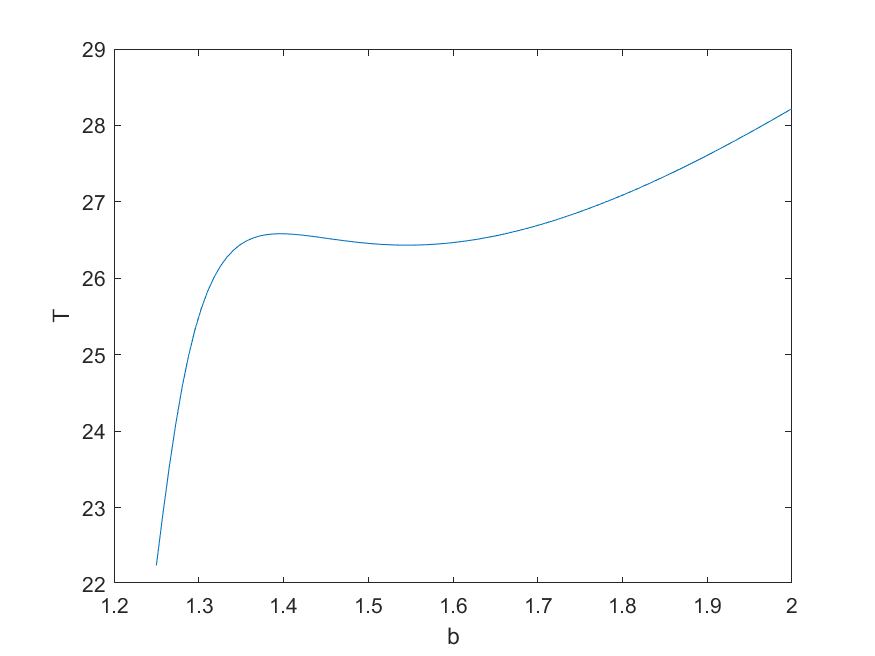
\includegraphics[width=\linewidth]{Labs/local_period.png}
\caption{Период цикла в зависимости от $b$}
\label{cyclesPeriod1}
\end{figure}

\newpage
Следующие два рисунка показывают зависимость координат $x$ и $y$ в зависимости от времени пи значениях $b = 1.31$ и $b = 5$.
Можно заметить, что движение вдоль оси $OX$ (от $M_0$ к $M_1$) замедляется, с ростом $b$, в то время как движение по <<гипотенузе>> и вдоль оси $OY$ ускоряется.
\begin{figure}[!h]
\minipage{0.55\textwidth}
\centering
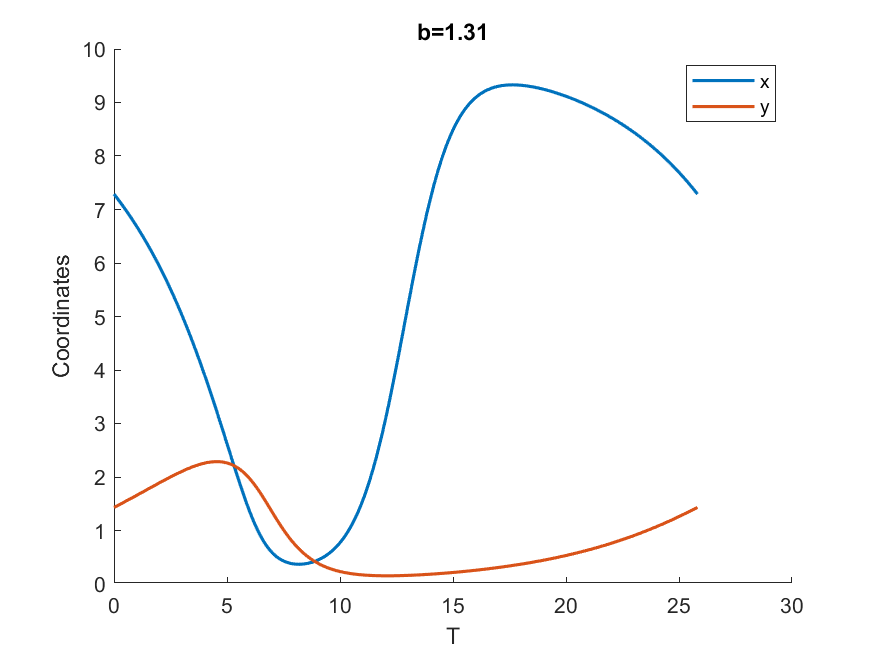
\includegraphics[width=\linewidth]{Labs/small_cycle.png}
\endminipage
\minipage{0.55\textwidth}
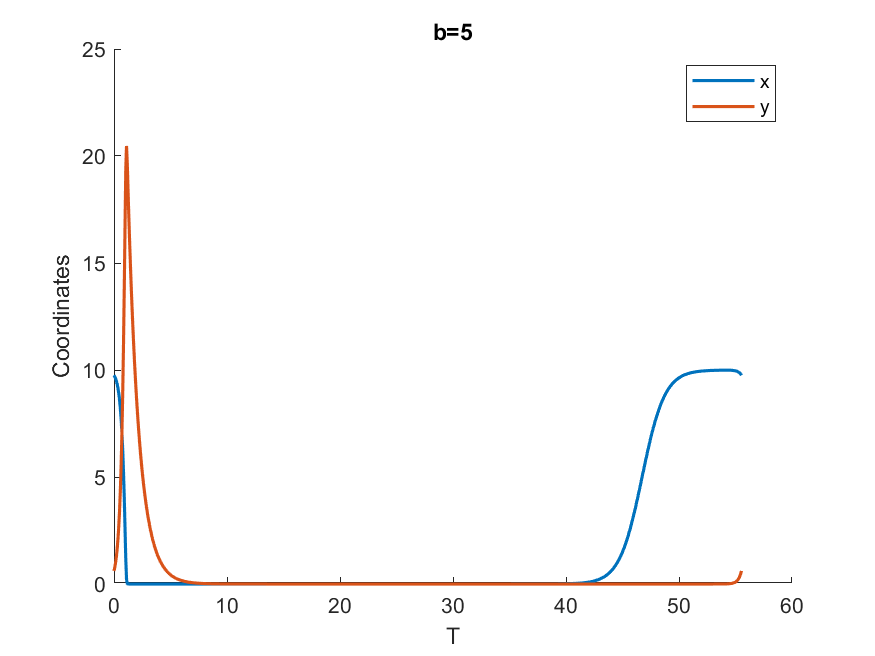
\includegraphics[width=\linewidth]{Labs/big_cycle.png}
\endminipage
\caption{Зависимость временных рядов от параметра $b$}
\label{cyclesPeriod2}
\end{figure}


\newpage
\section{Стохастические свойства модели}
\subsection{Моделирование случайных возмущений}
Для дальнейшего исследования свойств системы (1) внесем в её поведение случайные возмущения. Для этого, при построении траекторий системы, на каждом шаге метода численного интегрирования Рунге~--~Кутта 4 порядка будем добавлять к результату метода некоторую случайную добавку вида $\varepsilon  \sqrt{h} \xi$, где $\xi$ --- нормально распределённая случайная величина, $h$ --- шаг численного метода, $\varepsilon$ --- положительное число, коэффициент, регулирующий интенсивность возмущений.

Т.к. точки $M_0$ и $M_1$ имеют к 0 ординату, то шум у их окрестности будет покрывать отрицательные значения, что не имеет смысла для данной модели. Исследовать случайные возмущения будем только у оставшейся точки $M_2$.

\begin{figure}[!h]
\centering
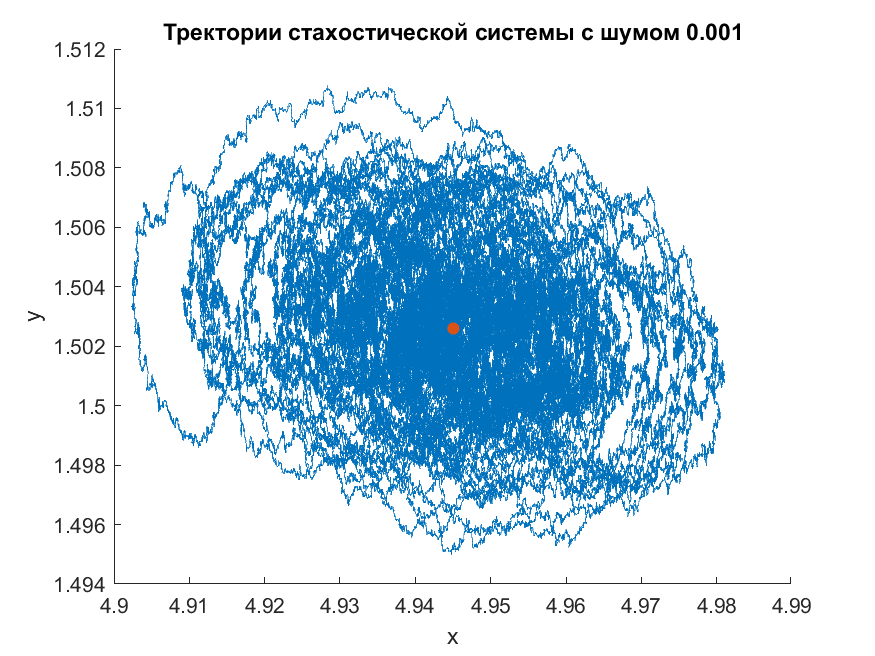
\includegraphics[scale=0.7]{Labs/stochastic_focus.png}
\caption{В окрестности фокуса $(b=1.22)$}
\label{sotch_focus}
\end{figure}

\newpage
\subsection{Возмущения в окрестности устойчивой точки покоя}
При внесении возмущений в траектории, стартующие в окрестности устойчивой точки покоя, траектории остаются в окрестности точки покоя при достаточно сильных шумах (рис. 16-17). 


\begin{figure}[!h]
\centering
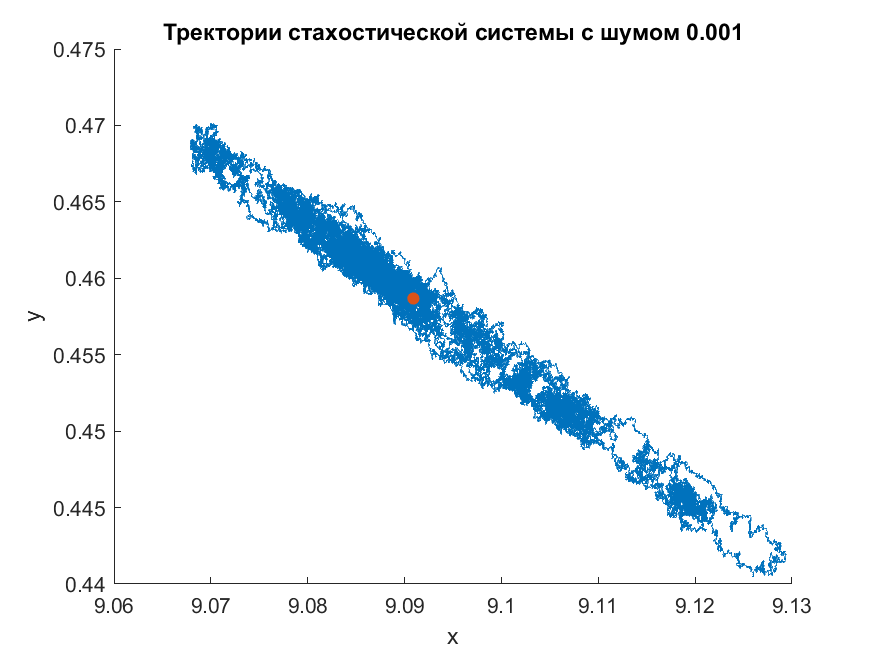
\includegraphics[width=\linewidth]{Labs/stochastic_node.png}
\caption{В окрестности узла $(b=1.11)$}
\label{sotch_node}
\end{figure}

\newpage
\begin{figure}[!h]
\centering
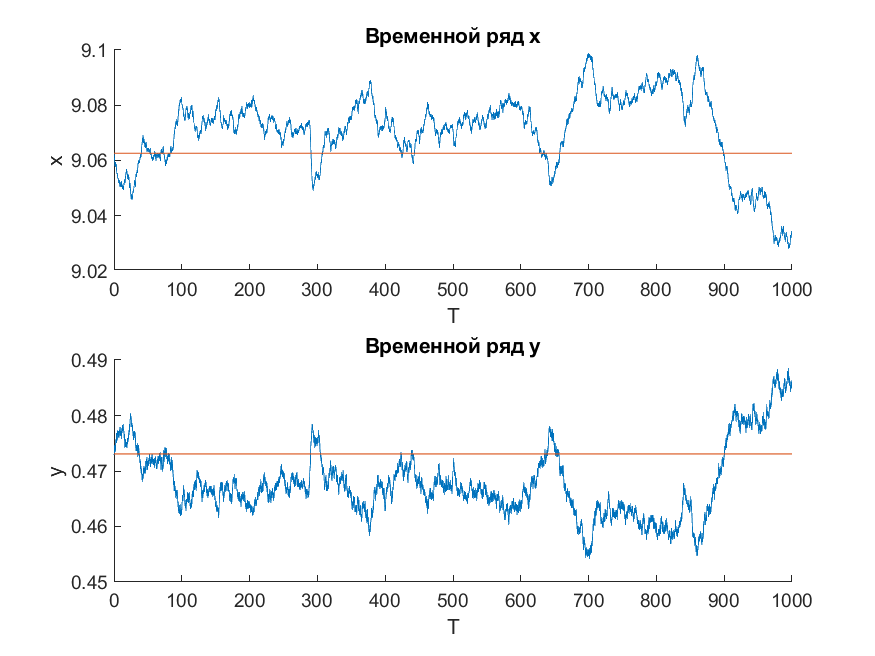
\includegraphics[width=\linewidth]{Labs/stochastic_node_coords.png}
\caption{Зависимость координат траекторий от времени}
\label{sotch_node_coord}
\end{figure}

На рисунке 18 можно заметить, что есть некая зависимость между отклонением от устойчивой точки для координат $x$ и $y$. В частности, блуждания имеют разные направления, а их величины отличаются в определенное число раз.

\newpage
\subsection{Матрица ковариации}
Деформацию распределения около точки устойчивого равновесия помогает объяснить матрица ковариации.
Значения собственных чисел матрицы говорят о размерах побочной и главной диагоналей эллипса, в котором находятся траектории блужданий. 
Т.к одно из собственных чисел матрицы близко к 0, то наблюдается растянутость элипса вдоль одной оси. (рис. 17)

\begin{figure}[!h]
\centering
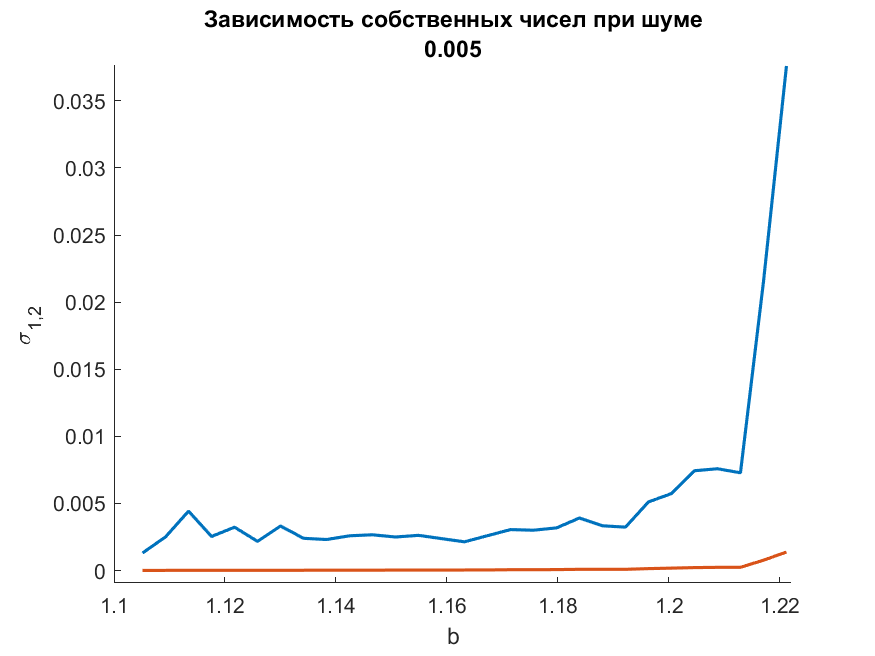
\includegraphics[scale=0.8]{Labs/singular.png}
\caption{Зависимость собственных чисел от параметра $b$}
\label{sotch_singular}
\end{figure}

\newpage
\subsection{Стохастический переход между аттракторами}
В данной системен не наблюдаются стохастические переходы между аттракторами.
Аттрактор либо один, либо находится очень близко к нулю, поэтому аддитивный шум не дает результата.

\newpage
\subsection{Возмущения в окрестности предельного цикла}
Рассмотрим влияние стохастических возмущений в окрестности предельного цикла. 

\begin{figure}[!h]
\centering
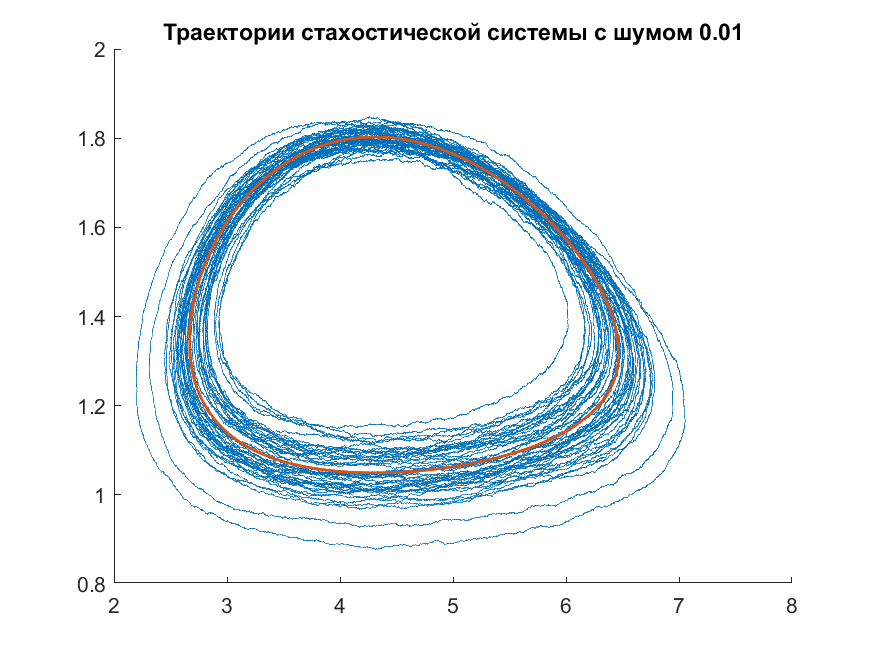
\includegraphics[width=\linewidth]{Labs/stochastic_cycle.png}
\caption{В окрестности цикла}
\label{sotch_node}
\end{figure}

\newpage
\begin{figure}[!h]
\centering
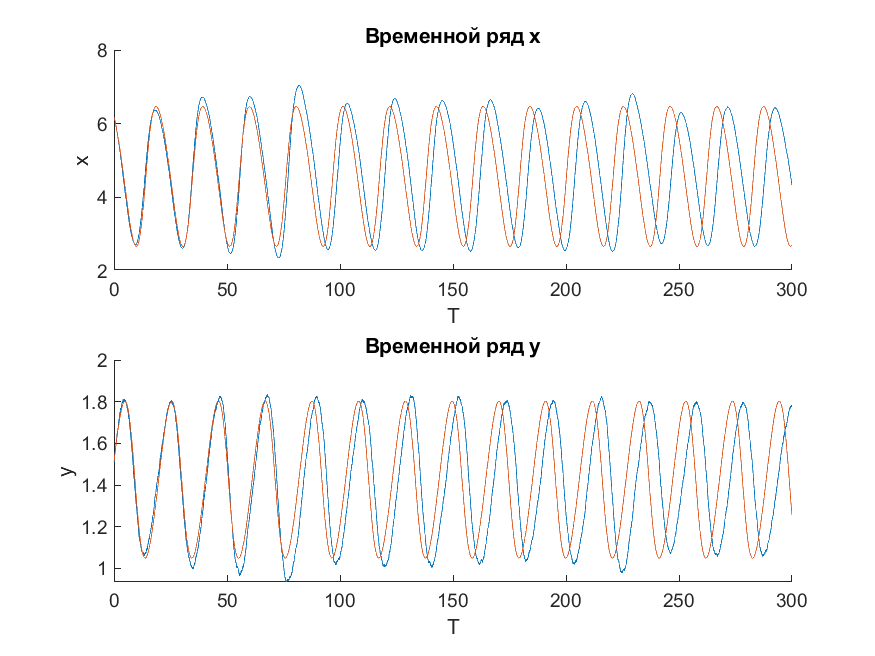
\includegraphics[width=\linewidth]{Labs/stochastic_cycle_coords.png}
\caption{Зависимость координат блужданий от времени}
\label{sotch_node_coord}
\end{figure}

\newpage
\begin{figure}[!h]
\centering
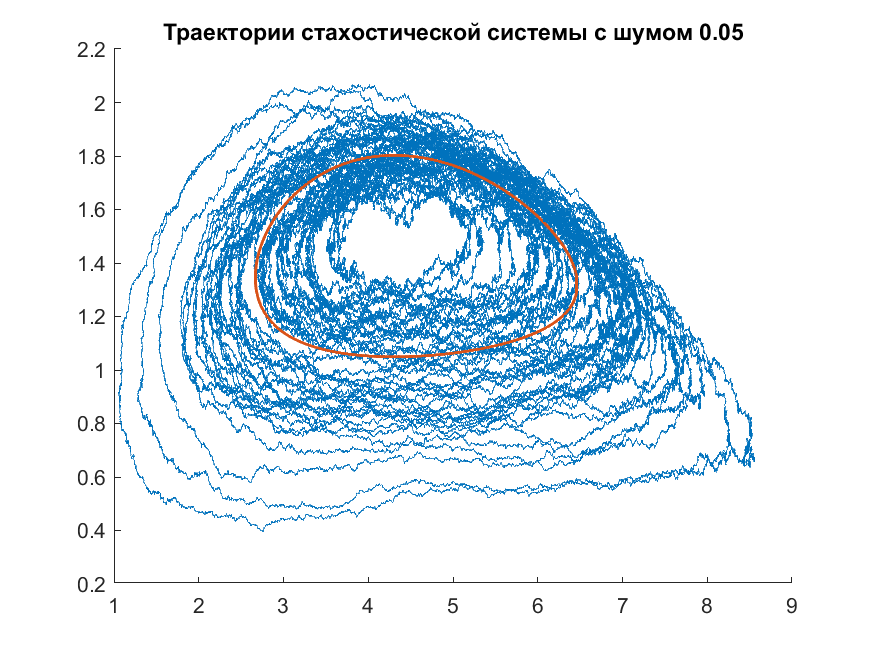
\includegraphics[scale=0.7]{Labs/stochastic_cycle_loud.png}
\caption{Возмущения в окрестности цикла с большим шумом}
\label{stoch_cycle_load}
\end{figure}

\begin{figure}[!h]
\centering
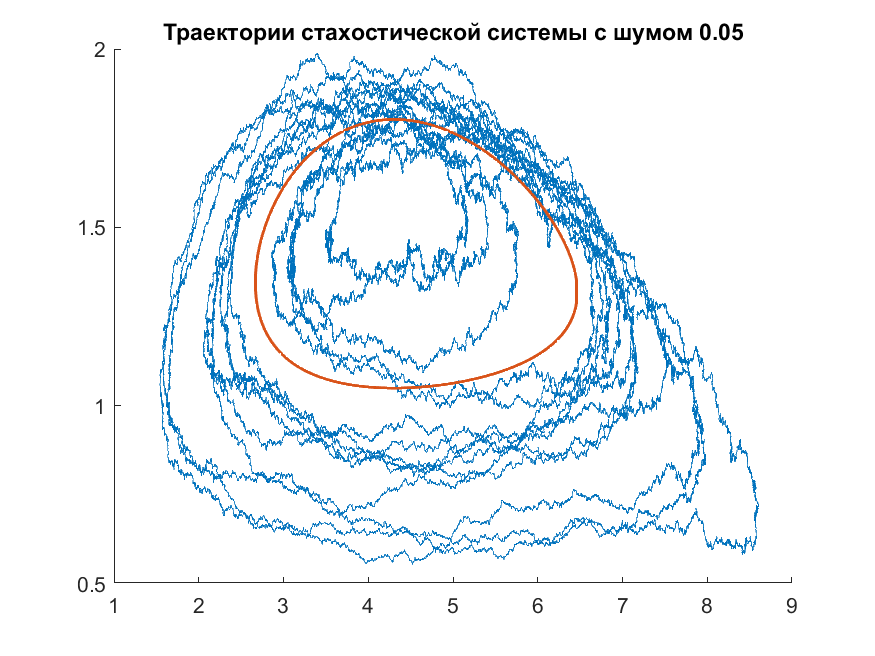
\includegraphics[scale=0.7]{Labs/stochastic_cycle_loud_2.png}
\caption{Возмущения в окрестности цикла с большим шумом}
\label{stoch_cycle_load}
\end{figure}


\newpage
\section{Заключение}
В процессе работы были изучены аттракторы системы, и рассмотрена их устойчивость; было показано, что  система имеет три точки покоя: 
независимую от параметров $ M_0 = \left(0,0 \right) $, 
независимую от насыщаемости хищника $ M_1 = \left(\dfrac{1}{c}, 0 \right) $ 
и зависимую от всех параметров $ M_2 = \left(\dfrac{1}{b-1}, \dfrac{(b-c-1)b}{a(b-1)^2} \right) $.

С помощью метода Рунге-Кутта были исследованы предельные циклы и показана их устойчивость.
Составлен атлас фазовых портретов. В зоне предельных циклов были исследованы орбиты циклов и их периоды. 

Для устойичивой точки покоя получены облака случайных состояний, проанализированы соответсвующие им временные ряды.
Показано влияние собственных чисел матрицы ковариаций на вид облаков.Индуцированные шумом осцилляции не обнаружены. 

В совокупности эти результаты позволяют судить о поведении системы и её траекторий, а также показывают, что при изменении значений параметров свойства нелинейных систем вообще и модели <<хищник-жертва>> Базыкина в частности могут значительно изменяться, возможно даже появление новых эффектов.

\newpage
\section{Бибилиография}
\begin{thebibliography}{5}
\bibitem{Chaos} Bashkirtseva I., Ryashko L. Sensitivity analysis of stochastic attractors and noise-induced transitions for population model with Allee effect // Chaos, 2011, V.21, p. 047514
\bibitem{Volterra}
Вольтерра В. Математическая теория борьбы за существование. Москва-Ижевск:, Институт компьютерных технологий, 2004. — 288 с.
\bibitem{Bashkirtseva} Башкирцева И.А., Перевалова Т.В. Анализ стохастических аттракторов при бифуркации точка покоя – цикл. // Автоматика и телемеханика. 2007. №10. C.53-69
\bibitem{Kriksunov} Криксунов Е.А., Пасечник В.В., Сидорин А.П. Экология. – М.: Издательский дом «Дрофа», 2010 г.
\end{thebibliography}

\end{document}